\begin{figure*}
  \centering
  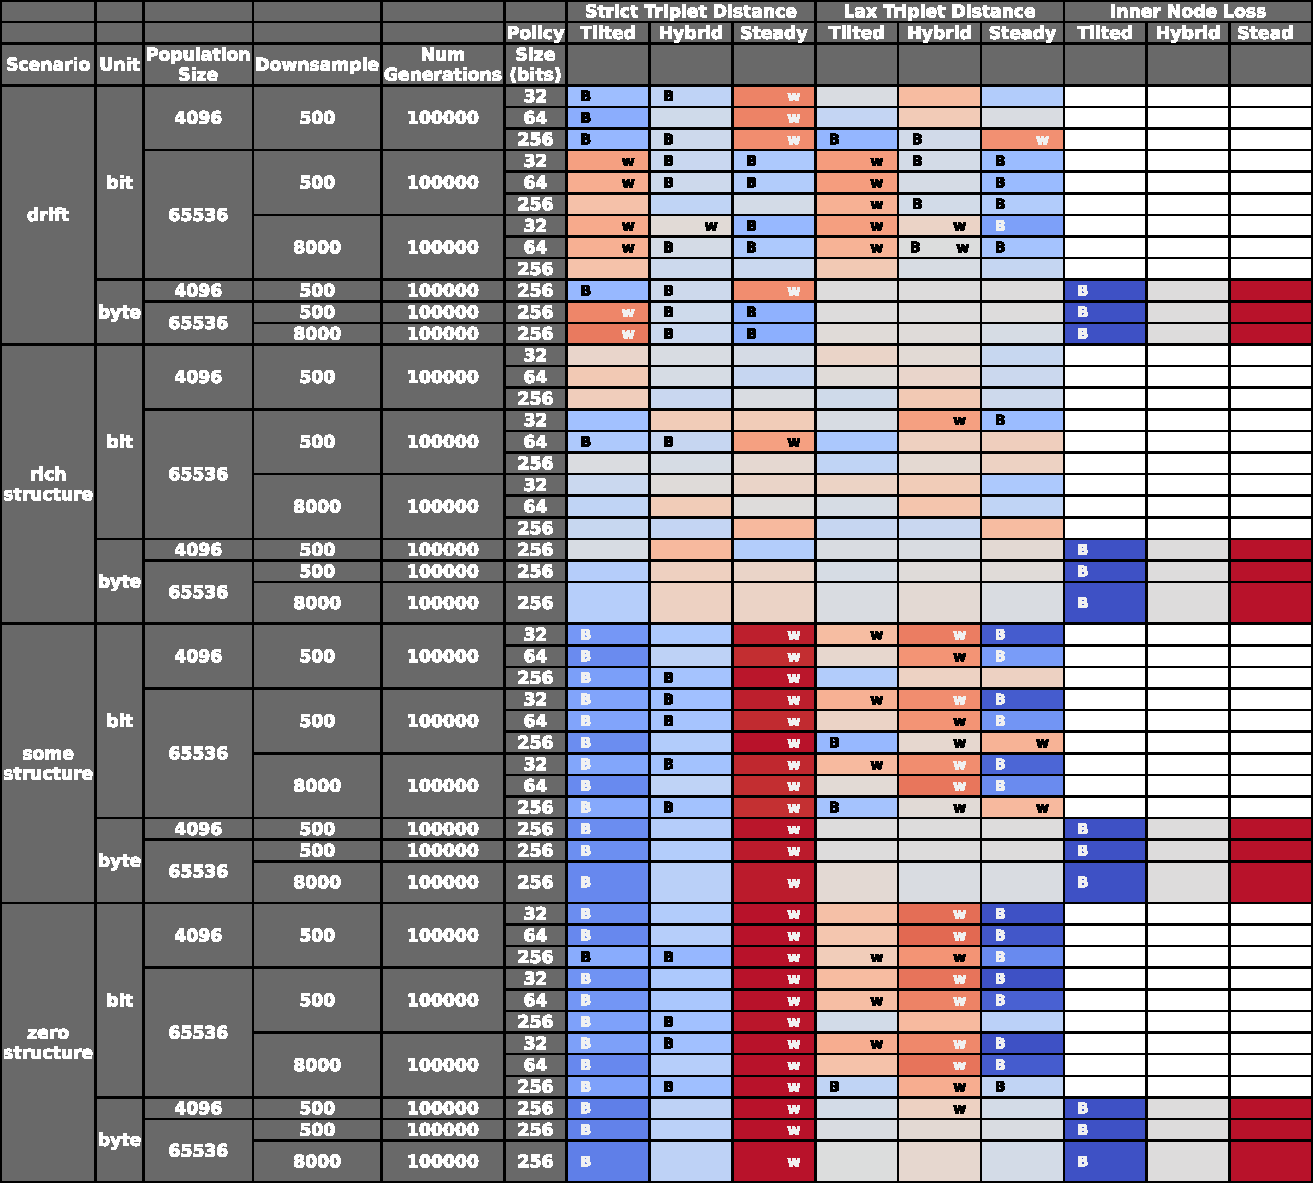
\includegraphics[width=\textwidth]{binder/binder/steady-vs-tilted/outplots/steady-vs-tilted-value}
  \caption{%
    \textbf{Comparison of reconstruction qualities under different differentia retention strategies.}
    \footnotesize
    Steady retention experiments used column-based implementation; tilted and hybrid retention experiments used surface-based implementation.
    For heatmap charts, B's indicate significantly best and w's significantly worst.
    Heatmap coloring is nonparametric mean rank among the three algorithms, with blue best and red worst.
  }
  \label{fig:steady-vs-tilted}
\end{figure*}
